\subsection{Advection Equation}\label{sec:advection}
\subsubsection{Problem Formulation}
We first consider the one-dimensional linear advection equation, with discontinuous residual $f$.
The problem has a simple analytical solution, serving as a sanity check for whether our implementation of the method has any merit.
The problem is defined by \eqref{eq:advection} below.
\begin{equation}
\begin{cases}
    u_t + \alpha \cdot u_x= 0 &\text{for } (x,t)\in [-1, 1] \times (0, 1] \\ 
    u(x, 0) = u_0(x)= f &\text{for } x \in [-1, 1],
\end{cases}
\label{eq:advection}
\end{equation}
where $\alpha = 0.5$, and the initial condition $f$ is defined by
\begin{equation*}
    f(x) =
    \begin{cases}
        1 &\text{if} \, x \in [-0.2, 0.2] \\
        0 &\text{else}.
    \end{cases}
\end{equation*}

By the method of characteristics, the analytical solution is:
\begin{equation}
    u(x,t) = u_0(x-\alpha t)=
    \begin{cases}
        1 &\text{if} \, x \in [-0.2 + \alpha t, 0.2 + \alpha t] \\
        0 &\text{else}.
    \end{cases}
\end{equation}

Thus, the problem defines a wave travelling rightwards without diffusion with a speed $\alpha$. The analytical solution also predicts two discontinuities. For our XPINN formulation, we decompose the domain according to the predicted discontinuities as in figure \textcolor{red}{Insert citation}.
In order to verify that our method is not simply learning the decomposition itself, we also verify that the wave is able to travel across the interfaces by setting $\alpha = 1$ while keeping the same decomposition.

Our network is composed of $6$ hidden layers, each with $20$ nodes, using $\tanh$ as our hidden activation function and no activation for the output layer.
We utilize $2000$ points for the interior, and $200$ evenly spread around the boundary and interfaces. 

\subsubsection{Results}

\subsection{Poisson Equation}
\subsubsection{Problem Formulation}
In this subsection, we consider a two-dimensional Poisson equation with residual discontinuity. The problem is a second order linear PDE, and is defined as:
\begin{align}\label{eq:poisson}
\begin{cases}
    u_{xx}+u_{yy} &= f \text{ on } \Omega \\
    u(x,y) &= 0 \text{ on } \partial\Omega,
\end{cases}
\end{align}
where $\Omega = (0,1) \times (0,1)$. For the Poisson problem, we consider two residuals. 
\paragraph{Continuous Residual:}
The first residual is given by:
\begin{equation}
    f_{cont}(x,y)= -2\pi^2\sin(\pi x) \sin(\pi y),
    \label{eq:continuous_poisson}
\end{equation}
which yields a known analytical solution:
\begin{equation*}
    u_{true}(x,y)=\sin(\pi x) \sin(\pi y).
\end{equation*}

Our experimental setup follows that of \textcite{müller2023achieving}.
We consider the problem for both a single PINN and for an XPINN decomposition shown in \autoref{fig:decomp_poisson}.
For the PINN, we train using 900 interior points and 120 boundary points distributed uniformly.
For the XPINNs, we also add 80 uniformly distributed interface points. We apply unitary weights to the boundary and interface losses.
Both solvers are trained using the \textsc{Adam} optimizer with an exponentially decreasing learning rate.
The initial learning rate is $10^{-3}$.
After $1.5\times 10^4$ steps, we decrease the learning rate by a factor of $10^{-1}$ every $10^4$ steps until a minimum learning rate of $10^{-7}$.
We train both cases for $2\times 10^5$ iterations. For our testing, we consider a uniform grid with 1,000,000 points. 


\begin{figure*}[t]
    % \centering
    \subfloat[PINN]{
    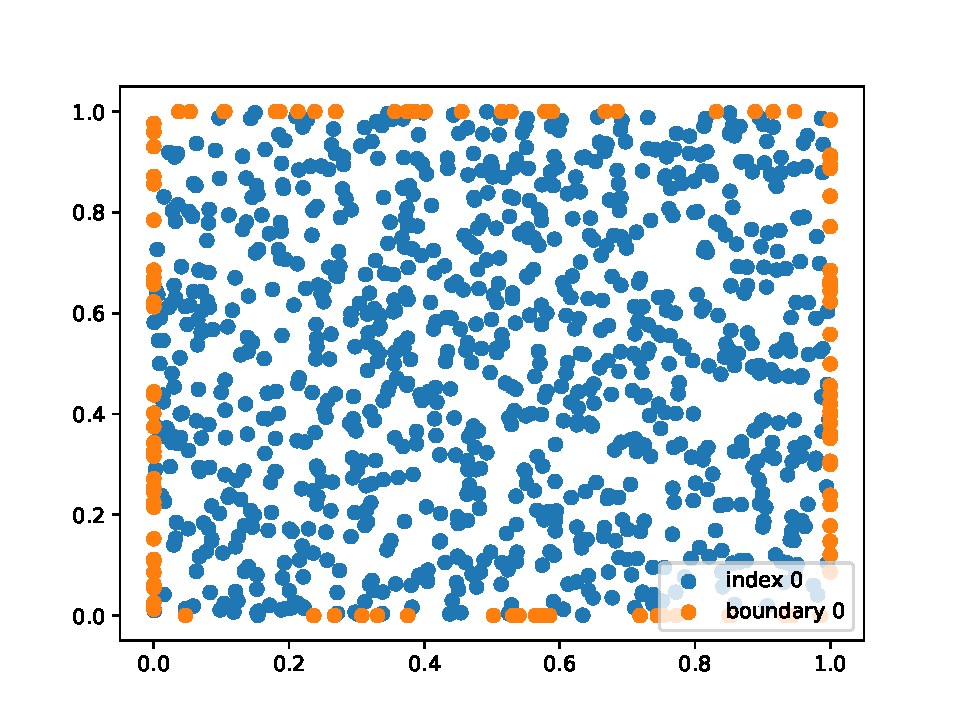
\includegraphics[width=0.48\textwidth]{Project1XPINNs/figures/Poisson/single_pinn_decomp.pdf}
    \label{subfig:single}
    }
    \hfill
    \subfloat[XPINN]{
    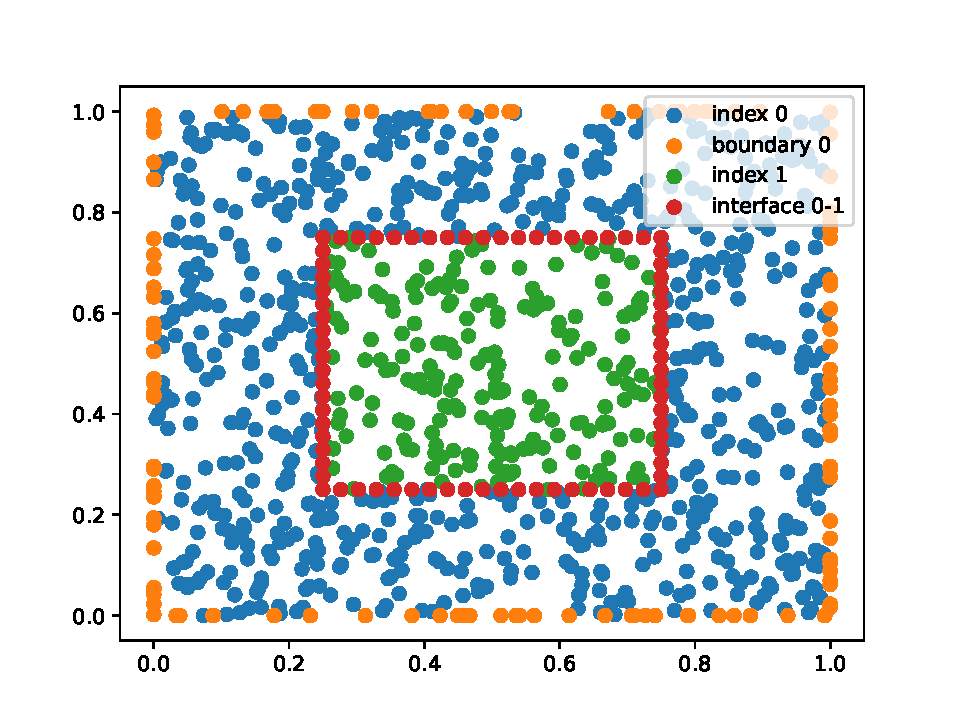
\includegraphics[width=0.48\textwidth]{Project1XPINNs/figures/Poisson/xpinn_decomp.pdf}
    \label{subfig:xpinn_decomp}
    }
    \caption{Example training points for the Poisson problem for a single PINN across the domain (left) and an XPINN where we have on PINN confined in the square $[0.25, 0.75]\times [0.25, 0.75]$ and the other for the remaining points. In both cases, we define 900 internal points and 120 boundary points. For the XPINN, we define an additional 80 interface points.}
    \label{fig:decomp_poisson}
\end{figure*}

\paragraph{Discrete Residual:}
The second residual is due \cite{XPINN_generalize}, where they compare the generalizeability of PINNs and XPINNs. We aim to reproduce their results. The residual is given as a discrete form:
\begin{equation*}
    f_{disc}(x,y)=
    \begin{cases}
        1 &\text{if} \, (x,y)\in [0.25,0.75]\times[0.25,0.75], \\
        0 &\text{else}.
        \label{eq:discrete_poisson}
    \end{cases}
\end{equation*}
Using our XPINN methodology, we aim to reproduce the results presented by \textcite{XPINN_generalize}.

\subsubsection{Results}
\paragraph{Continuous Residual:}
\autoref{table:cont_poisson} shows the minimum, median, and maximum relative $L^2$ errors of the single PINN and XPINN solvers for the continuous residual Poisson equation using the \textsc{Adam} optimizer. Note that the mesh was re-generated between each iteration. Note the significant improvement in the $L^2$
\begin{table}[h]
\caption{Median, minimum and maximum of the relative $L^2$-errors for the Poisson equation with continuous residual achieved by the single PINN and our XPINN decomposition. }
    \centering
    \begin{tabular}{|l|l l l|}
    \hline
     & Median & Minimum & Maximum
    \\
    \hline
    PINN &$1.5\cdot 10^{-3}$ &  $7.70 \cdot 10^{-4}$&$2.55 \cdot 10^{-3}$ 
    \\
    XPINN &\(s_{i, j-1}\) & \(s_{i, j}\) & \(s_{i, j+1}\)
    \\
    \hline
    \end{tabular}
    \label{table:cont_poisson}
\end{table}


\subsection{Navier-Stokes Equation}
\subsubsection{Problem Formulation}
Finally, we consider the Navier Stokes problem as described in \textcolor{red}{cite benchmark}. This problem is a simulation of an incompressible 2D fluid flow hitting a cylinder in a rectangle. In the DFG benchmark 2D-1, the PDE conditions are given by:
\begin{equation}
    -\nu \nabla^2 \mathbf{u} + (\mathbf{u} \cdot \nabla)\mathbf{u} + \nabla p = \mathbf{0}, \hspace{3mm} \nabla \cdot \mathbf{u} = 0
\end{equation}
where $\nu = 0.001$. In our notation, we will isolate the x- and y-flow as $u$ and $v$ respectively. From this, we can express the PDEs for the second-order spatial derivatives, as well as the equation for zero convergence due to incompressibility as
\begin{equation}
\begin{cases}
-\nu(u_{xx} + u_{yy})+uu_x+vu_y+p_x = 0 \\
-\nu(v_{xx} + v_{yy})+uv_x+vv_y+p_y = 0 \\
u_x + v_y = 0
\end{cases}
\end{equation}
In order to impose the zero divergence condition, we let our network $\mathcal{N}_\theta$ predict both the stream function $\psi$ and the pressure $p$.
\begin{equation}
    \mathcal{N}_\theta : \mathbb{R}^3 \to \mathbb{R}^2, \quad (x,y,t)\to (\psi, p)
\end{equation}
We obtain $u$ and $v$ from the equations $u=\psi_y$ and $v=-\psi_x$. \\
This problem includes three different boundary conditions. First, we have the boundary for the upper and lower walls, as well as around the edge of the cylinder. On these walls, we require the flow to be exactly zero. In the DFG benchmark 2D-1 \textcolor{red}{cite benchmark}, the lower and upper walls are notated as $\Gamma_1 = [0,2.2]\times 0$ and $\Gamma_3 = [0,2.2]\times 0.41$ respectively, and the boundary as $S=\partial B_r(0.2,0.2)$. The no-slip boundary condition is defined as
\begin{align*}
    u_{|\Gamma_1} = u_{|\Gamma_3} = u_{|S} &= 0 \\
    v_{|\Gamma_1} = v_{|\Gamma_3} = v_{|S} &= 0
\end{align*}
On the left boundary we enforce polynomial inflow. The left boundary is $\Gamma_2 = 0\times [0,0.41]$ and the polynomial inflow is given by
\begin{equation*}
    u=\frac{4Uy(0.41-y)}{0.41^2}, \quad v=0
\end{equation*}
where $U=0.3$
Finally, on the right boundary we have the do-nothing boundary condition. The boundary is $\Gamma_4=2.2\times[0,0.41]$, and the condition is given by
\begin{equation*}
    \nu u_x - p = 0, \quad \nu u_y = 0
\end{equation*}
\subsubsection{Results}
